No repositório \colorurl{https://github.com/j-Lago/pythonTutorial/blob/master/data/} você encontrará o
arquivo \colorurl{subestacao.csv}, que contém medições de
diversas grandezas elétricas registradas por um analisador de potência instalado na subestação de uma empresa da região.

Os dados foram registrados em intervalos de 10 minutos, representando métricas estatísticas
(como média, valor máximo e mínimo) calculadas para cada janela de amostragem, ao longo de um período de duas semanas.

Importe os dados para um \inlcode{pandas.DataFrame}, realize uma análise que gere um gráfico com o consumo
médio por hora do dia, destacando o horário que, em média, tem o maior consumo.

Considere apenas os dias úteis, desconsiderando os finais de semana.

A \figr{fig:subestacao} mostra um exemplo de como os resultados do script podem ser apresentados.
\begin{figure}[htbp]
    \centering
    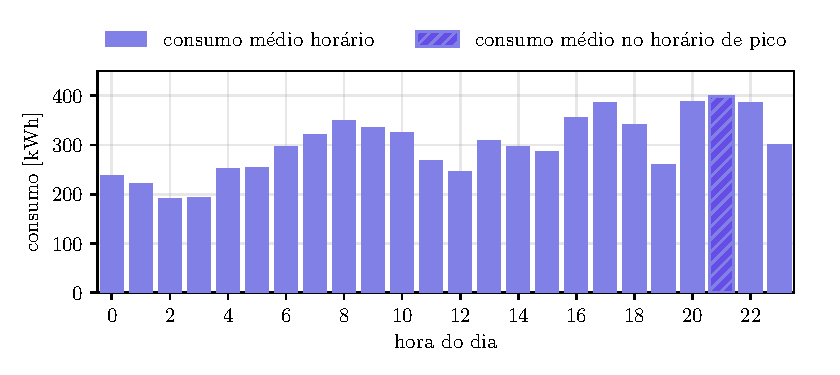
\includegraphics[scale=1.0]{figs/subestacao}
    \caption{Resultado esperado.}
    \label{fig:subestacao}
\end{figure}

\subsection*{Dica:}
A primeira coluna do arquivo representa um \emph{timestamp} das amostras e, por isso, é recomendável utilizá-la
como \inlcode{index} do \inlcode{DataFrame}.
Ao converter esses valores de \emph{timestamp} para o tipo \inlcode{datetime} (que, por padrão, seriam importados
como \inlcode{str}), você passa a contar com métodos
bastante úteis da API de datas e horas do \inlcode{pandas}, como \inlcode{.hour}, \inlcode{.weekday}, entre outros ---
o que pode facilitar significativamente a análise temporal requerida neste exercício.
\begin{minted}{custompython}
df = pd.read_csv('subestacao.csv',
                 index_col='time', parse_dates=['time'], date_format='%Y-%m-%d %H:%M:%S')
\end{minted}